% !TEX root =  ../../master.tex
\subsection{Grundgerüst}

Um auf den einzelnen Unterseiten der Anwendung einen Anhaltspunkt zu besitzen, ist die Abbildung \ref{fig:MockGrundgeruest} da. 
In dieser wird eine grundlegende Struktur festgelegt, welche auf den Unterseiten der Webanwendung verwendet werden soll.
Dabei wird die Seite in unterschiedliche Sektoren untergliedert.
Die einzelnen Komponenten einer Seite sind dabei der \emph{Header}, \emph{Inhalt der Seite}, sowie der \emph{Footer}. 
Wie schon die Namen der Sektoren indizieren, ist die Anordnung von \emph{Header} über den \emph{Inhalt der Seite} zu dem abschließenden \emph{Footer}, strukturiert.
Jedoch besitzen diese Komponenten nicht die maximale Breite.
Daher gibt es an den rechten und linken Rand der Seite jeweils ungenutzte Fläche. 
Diese freie Fläche ist jedoch gewollt, dadurch soll der Benutzer nicht mit zu viel Inhalt auf einmal konfrontiert werden.
Somit kann seine Aufmerksamkeit auf den \emph{Inhalt der Seite} gelenkt werden.
Als Vorteil besitzt ein konsistenter Aufbau, dass sich der Benutzer an eine Struktur gewöhnen kann. 

\begin{figure}[H]
	\centering
	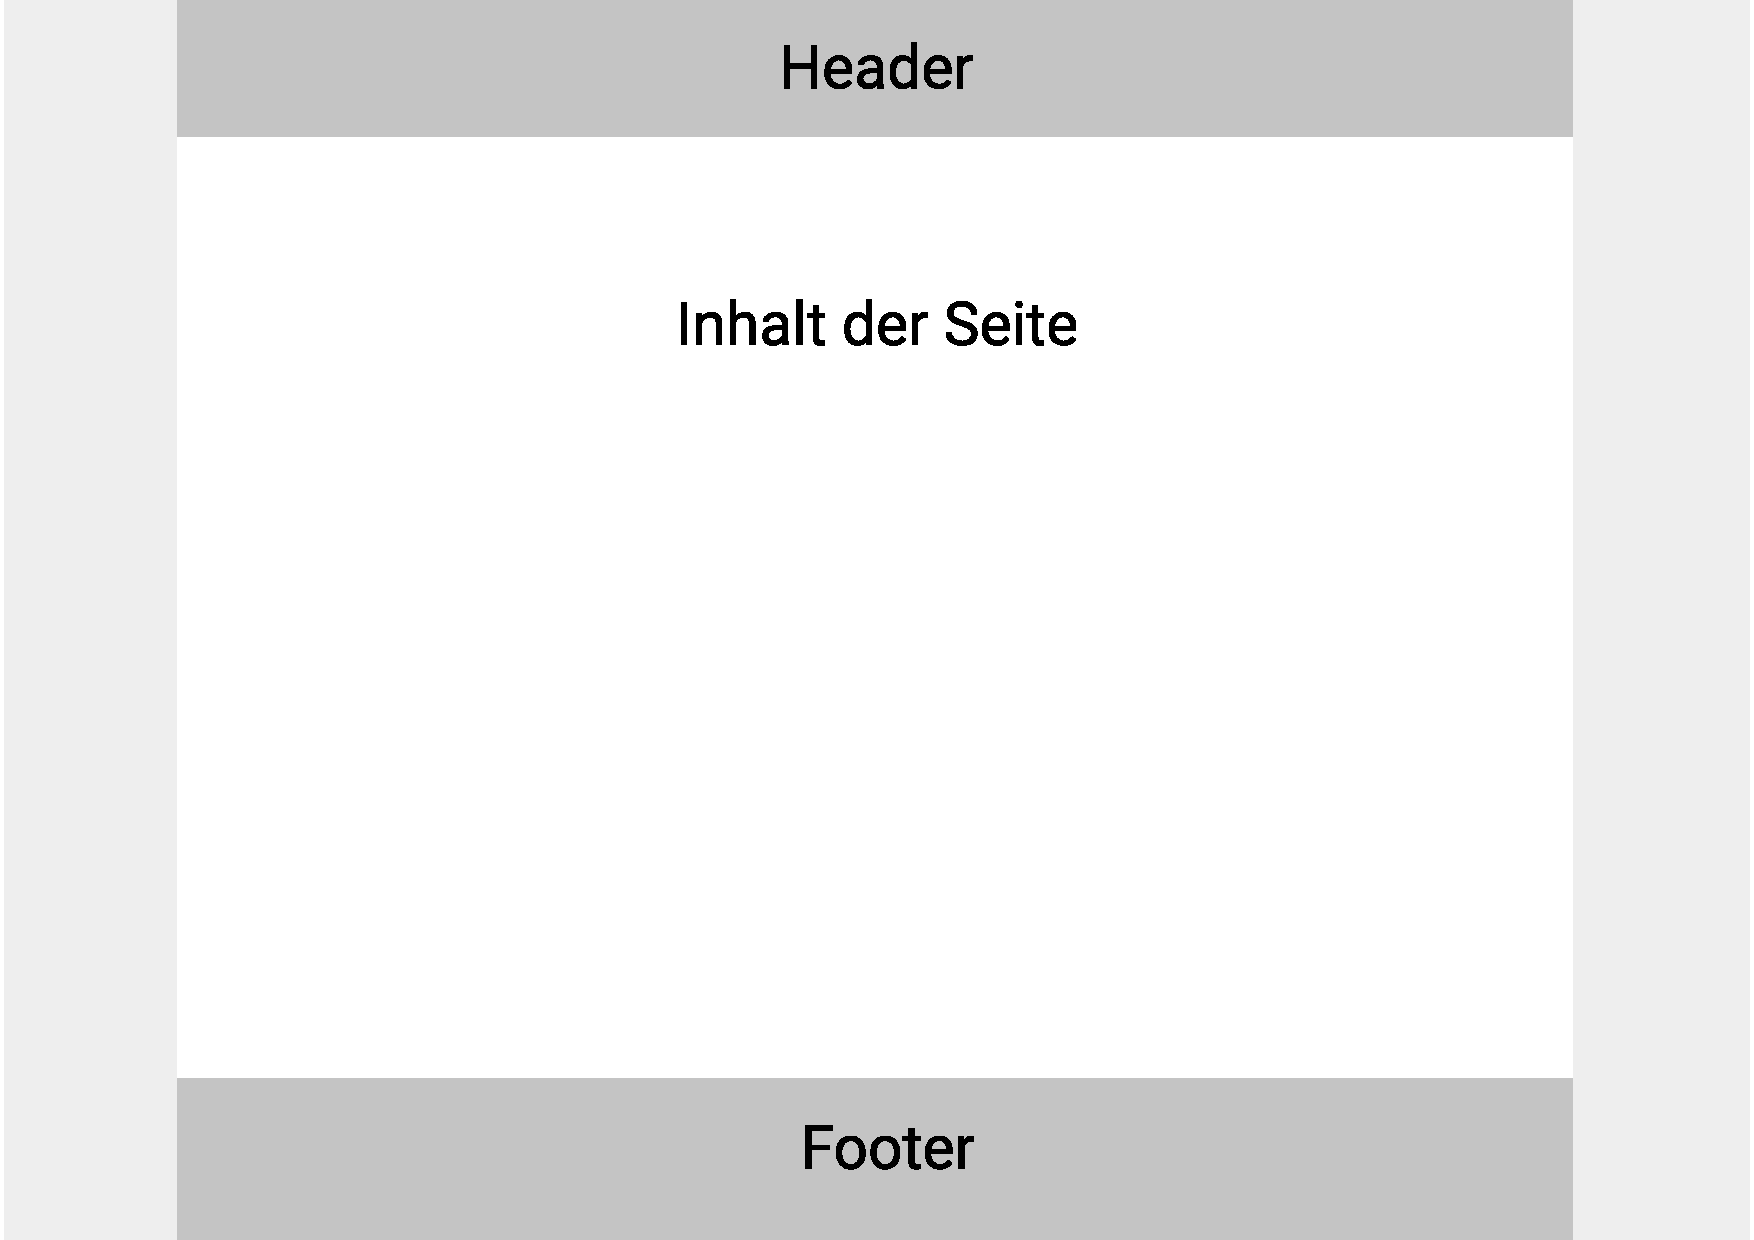
\includegraphics[width=0.7\textwidth]{img/konzeption/client/grundgeruest}
	\captionsetup{justification=centering, format=plain}
	\caption[Mock-Up vom Grundgerüst der Anwendung]{Mock-Up vom Grundgerüst der Anwendung \\\figma}
	\label{fig:MockGrundgeruest}
\end{figure}
